\renewcommand{\theequation}{\theenumi}
\renewcommand{\thefigure}{\theenumi}
\renewcommand{\thetable}{\theenumi}
\begin{enumerate}[label=\thesection.\arabic*.,ref=\thesection.\theenumi]
\numberwithin{equation}{enumi}
\numberwithin{figure}{enumi}
\numberwithin{table}{enumi}

\item Two random variables X and Y are distributed according to\\
{\centering $
f_{x,y}(x,y) = 
\begin{cases}
 (x+y) & 0 \leqslant x \leqslant 1   0 \leqslant y \leqslant 1 \\
 0 & \text{otherwise}.
 \end{cases}
 $ \\}
The probability $P(X+Y \leqslant 1)$ is .......
%

\item Let $X$ and $Y$ be two random variables having the joint probability density function

\begin{center}
$ 
f(x,y)=
\begin{cases}
2 &  \ 0<x<y<1 \\
0 & \text{otherwise}.
\end{cases}
$\\ 
\end{center}

Then the conditional probability $P \brak{X \leq\ \frac{2}{3} | Y=\frac{3}{4}}$ is equal to \underline{\hspace{3cm}}

\begin{enumerate}
\begin{multicols}{4}
\setlength\itemsep{2em}

\item $
\frac{5}{9}
$
\item $
\frac{2}{3}
$
\item $
\frac{7}{9}
$
\item $
\frac{8}{9}
$


\end{multicols}
\end{enumerate}

\item Let X and Y be jointly distributed random variables having the joint probability density function \\
$
f(x,y) = 
\begin{cases} 
\frac{1}{\pi} 
&  x^2+y^2 \leqslant 1 \\
0 & \text{otherwise}
\end{cases}
$ \\
Then $P(Y>max(X,-X))=$

\begin{enumerate}
\begin{multicols}{2}
\setlength\itemsep{2em}

\item $\dfrac{1}{2}$
\item $\dfrac{1}{3}$
\item $\dfrac{1}{4}$
\item $\dfrac{1}{6}$

\end{multicols}
\end{enumerate}
\solution
pdf of $X$ is :
\begin{align}
    f_X(x)&=\int_{-\infty}^{\infty}f(x,y)dy\\
    &=\int_{-\sqrt{1-x^2}}^{\sqrt{1-x^2}}\frac{1}{\pi}dy\\
    &=\frac{2\sqrt{1-x^2}}{\pi}
\end{align}
pdf of $Y$ is :
\begin{align}
    f_Y(y)&=\int_{-\infty}^{\infty}f(x,y)dx\\
    &=\int_{-\sqrt{1-y^2}}^{\sqrt{1-y^2}}\frac{1}{\pi}dx\\
    &=\frac{2\sqrt{1-y^2}}{\pi}
\end{align}
cdf of $Y$ is:
\begin{align}
    F_Y(y)&=\int_{-\infty}^{y}f_Y(y)dy\\
    &=\int_{-1}^{y}\frac{2\sqrt{1-y^2}}{\pi}dy\\
    &=\frac{2}{\pi}\sbrak{\dfrac{\sin^{-1}{y} + y\sqrt{1-y^2}}{2} + \frac{\pi}{4}}
\end{align}
The value of $\pr{-X<Y<X}$ is:
\begin{align}
\pr{-X<Y<X} &=F_Y(X)-F_Y(-X)\\
 &=\frac{2}{\pi}\brak{\sin^{-1}{X} + X\sqrt{1-X^2}}
\end{align}
Integrating our probability over all of $X$ we get the value of $ E[\pr{-x<Y<x}]$ as 
\begin{align}
&=\int_{-\infty}^{\infty}f_X(x)\pr{-x<Y<x}dx\\
    &=\brak{\frac{2}{\pi}}^2\int_0^1\sqrt{1-x^2}\brak{\sin^{-1}{x} + x\sqrt{1-x^2}}dx
\end{align}
Substituting
\begin{align} 
u &= \sin^{-1}{x} + x\sqrt{1-x^2}\\
\frac{du}{dx} &= 2\sqrt{1-x^2}\\
&=\brak{\frac{2}{\pi}}^2\int_0^{\frac{\pi}{2}}\frac{u}{2}du\\
&=\brak{\frac{2}{\pi}}^2\brak{\frac{u^2}{4}} \bigg |_0^{\frac{\pi}{2}}\\
&=\brak{\frac{2}{\pi}}^2\brak{\frac{\pi^2}{16} - 0}\\
    &=\frac{4\cdot{\pi}^2}{{\pi}^2\cdot16}\\
    &=\frac{1}{4}
    \end{align}

\begin{center}
    \centering\underline{\textbf{Common Data for the next two Questions :}}
    \end{center}
    
\item     Let X and Y be random variables having the joining probability density function \\
    $
    f(x,y)=
    \begin{cases}
    {\dfrac{1}{\sqrt{2 \pi y}}}e^{\frac{-1}{2y}(x-y)^2}
    & -\infty < x < \infty,\\  
    &  0 < y < 1
    \\
    0 & \text{otherwise}
    \end{cases}
    $ \\
    
    The variance of the random variable X is 
    
    \begin{enumerate}
    \begin{multicols}{2}
    \setlength\itemsep{2em}
    
    \item $\dfrac{1}{12}$
    \item $\dfrac{1}{4}$
    \item $\dfrac{7}{12}$
    \item $\dfrac{5}{12}$
    
    \end{multicols}
    \end{enumerate}
    
    \item The covariance between the random variables X and Y
    
    \begin{enumerate}
    \begin{multicols}{2}
    \setlength\itemsep{2em}
    
    \item $\dfrac{1}{3}$
    \item $\dfrac{1}{4}$
    \item $\dfrac{1}{6}$
    \item $\dfrac{1}{12}$
    
    \end{multicols}
    \end{enumerate}
    
        
\item         Let X and Y be continuous random variables with the joint probability density function \\
        
        $
        f(x,y)=
        \begin{cases}
        a{e^{-2y}}
        & 0 <x<y< \infty \\
        0 & \text{otherwise}
        \end{cases}
        $
        
        The value of a is
        
        \begin{enumerate}
        \begin{multicols}{2}
        \setlength\itemsep{2em}
        
        \item 4
        \item 2
        \item 1
        \item 0.5
        
        \end{multicols}
        \end{enumerate}
        
        \item The value of $E(X|Y=2)$ is
        
        \begin{enumerate}
        \begin{multicols}{2}
        \setlength\itemsep{2em}
        
        \item 4
        \item 3
        \item 2
        \item 1
        \end{multicols}
        \end{enumerate}
        
        \item Let X and Y be two random variables having the joint probability density function \\

        $
        f(x,y)=
        \begin{cases}
        2 &  0<x<y<1 \\
        0 & \text{otherwise}
        \end{cases}
        $ \\
        Then the conditional probability $P(X \leqslant {\frac{2}{3}}| Y={\frac{3}{4}})$ is equal to
        
        \begin{enumerate}
        \begin{multicols}{2}
        \setlength\itemsep{2em}
        
        \item $\dfrac{5}{9}$
        \item $\dfrac{2}{3}$
        \item $\dfrac{7}{9}$
        \item $\dfrac{8}{9}$
        \end{multicols}
        \end{enumerate}
        

            
\item             Let X and Y be two continuous random variables with the joint probability density function \\
            $
            f(x,y)= 
            \begin{cases}
            2 & 0<x+y<1, x>0, y>0 \\
            0 & \text{elsewhere}.
            \end{cases}
            $
            
            $P(X+Y<\frac{1}{2})$ is
            
            \begin{enumerate}
            \begin{multicols}{2}
            \setlength\itemsep{2em}
            
            \item $\dfrac{1}{4}$
            \item $\dfrac{1}{2}$
            \item $\dfrac{3}{4}$
            \item 1
            \end{multicols}
            \end{enumerate}
            %
            %
            \solution
            Given X and Y be two continuous random variables with the joint probability density function
\begin{align}
    f\left(x,y\right)=\begin{cases}
    2 \quad  0<x+y<1 ,x>0 ,y>0\\
    0 \quad  \textrm{elsewhere}\\
    \end{cases}
\end{align}
% \begin{figure}[h]
%     \centering
%     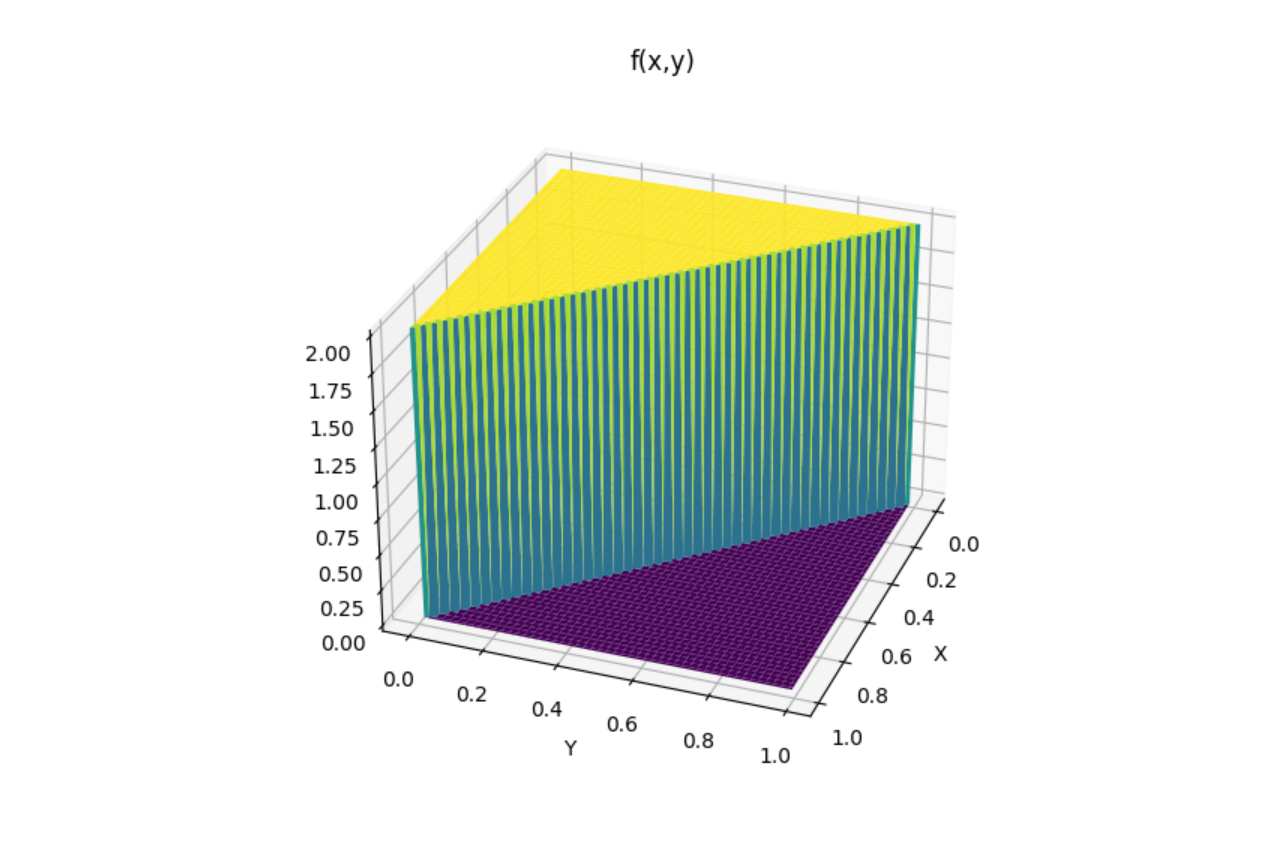
\includegraphics[scale=0.2]{f(x,y)_graph.png}
%     \caption{$f\left(x,y\right)$}
%     \label{ec/75/fig:f(x,y)}
% \end{figure}

we know that
\begin{align}
    P\left(\left(x,y\right)\in A\right)=\int \int _{A}f\left(x,y\right) dx dy \quad  A \in \mathbb{R}^2
\end{align}
from given information\\
for positive $x$ and $y$
\begin{align}
    0<x+y<\dfrac{1}{2}  \Rightarrow 0<x<\dfrac{1}{2}-y
\end{align}
so using eq(0.0.3)
\begin{align}
    P\left(x+y < \dfrac{1}{2}\right)=\int_{0}^{\frac{1}{2}} \int _{0}^{\frac{1}{2}-y}f(x,y) dx dy\\
    =\int_{0}^{\frac{1}{2}} \int _{0}^{\frac{1}{2}-y} 2 \quad dx dy
    =\int_{0}^{\frac{1}{2}} \left(  2 x \quad \big|_{0}^{\frac{1}{2}-y} \right)  dy\\
    =\int_{0}^{\frac{1}{2}}   2 \left(\frac{1}{2}-y\right) \quad    dy
    =2\left( \frac{1}{2} y - \frac{y^2}{2}  \right) \big|_{0}^{\frac{1}{2}}\\
    = \left( \frac{1}{2} - \frac{1}{4}\right) = \frac{1}{4} 
\end{align}
Therefore 
\begin{align}
    P\left(X+Y<\dfrac{1}{2}\right)=\dfrac{1}{4}
\end{align}
\begin{align}
\intertext{volume under the graph which contains the region} X+Y<\dfrac{1}{2} \quad \text{gives us} \quad P\left(X+Y<\dfrac{1}{2}\right) \\
 P\left(X+Y<\dfrac{1}{2}\right)= \text{Area of the base . height}
 \end{align}
 
Area of the base triangle is 
\begin{align}
 \dfrac{1}{2}.\textit{height}.\textit{base} =\dfrac{1}{2}.\dfrac{1}{2}.\dfrac{1}{2}
 \end{align}
 \begin{align}
\text{volume = Area . height}=\dfrac{1}{8}. 2= \dfrac{1}{4}
\end{align}
%The volume under the graph which contains the region $X+Y<\dfrac{1}{2}$ %gives us $P\left(x+y<\dfrac{1}{2}\right)$\\
%$P\left(x+y<\dfrac{1}{2}\right)=$ Area of the base . height\\
%Area of the base triangle is $\dfrac{1}{2}.\textit{height}.\textit{base}$%$= \dfrac{1}{2}.\dfrac{1}{2}.\dfrac{1}{2}$\\
%volume = Area . height $= \dfrac{1}{8}. 2= \dfrac{1}{4}$

\begin{figure}[h]
    \centering
    %\columnwidth
    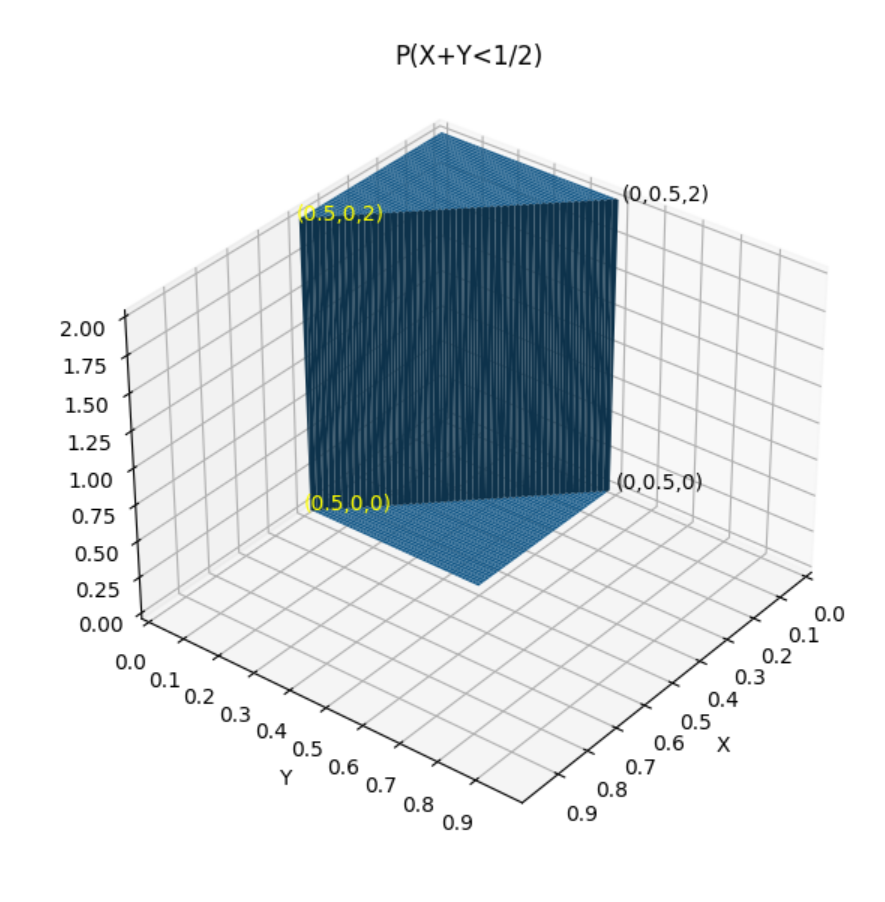
\includegraphics[width=\columnwidth]{solutions/ec/75/P(x+y_2)_graph.png}
    \caption{$P\left(x+y<\dfrac{1}{2}\right)$}
    \label{ec/75/fig:p(x+y<1/2)}
\end{figure}



            
            \item $E(X|Y=\frac{1}{2})$
            
            \begin{enumerate}
            \begin{multicols}{2}
            \setlength\itemsep{2em}
            
            \item $\dfrac{1}{4}$
            \item $\dfrac{1}{2}$
            \item 1
            \item 2
            \end{multicols}
            \end{enumerate}
            %
            \solution
            Let X and Y be two continuous random variables with the joint probability density function 
\begin{align}
f\brak{x,y}= 
\begin{cases}
2 & 0<x+y<1, x>0, y>0 \\
0 & \text{elsewhere}.
\end{cases}   
\end{align}
\\Then $E\brak{X|Y=\frac{1}{2}}$ is 
%
Given X and Y are two continuous random variables with joint probability density function,
\begin{align}
f\brak{x,y}= 
\begin{cases}
2 & 0<x+y<1, x>0, y>0 \\
0 & \text{elsewhere}.
\end{cases}    
\end{align}
\\We know that,\\
$0<x+y<1  \implies 0<y<1-x \text{ for } 0<x<1.$\\ 
Then,
\begin{align}
    f_X\brak{x} &= \int f_{XY}\brak{x,y}dy\\
    &= \int_{0}^{1-x} (2)dy\\
    &= 2(1-x)\\
\implies f_X\brak{x} &=
    \begin{cases}
    2(1-x) & 0 \leq x <1\\
    0 & \text{otherwise}.
    \end{cases}
\end{align}
Similarly,\\
$ 0<x+y<1 \implies 0<x<1-y \text{ for } 0<y<1$ \\
Then,
\begin{align}
    f_y\brak{y} &= \int f_{XY}\brak{x,y}dx\\
    &= \int_{0}^{1-y} (2)dx\\
    &= 2(1-y)\\
\implies f_Y\brak{y} &=
    \begin{cases}
    2(1-y) & 0 \leq y <1\\
    0 & \text{otherwise}.
    \end{cases}
\end{align}
Therefore ,
\begin{align}
    f_{X|Y}\brak{x|y} &= \frac{f_{XY}\brak{x,y}}{f_Y\brak{y}}\\
    & = 
    \begin{cases}
    \frac{2}{2(1-y)} & \text{if } 0\leq x+y < 1\\
    0 & \text{otherwise}
    \end{cases}
\end{align}
Then, 
\begin{align}
   E\brak{X|Y=y} & =
   \int_{-\infty}^{\infty} (x)\brak{\frac{1}{1-y}}dx\\
    & = \frac{1}{1-y} \int_{0}^{1-y}(x)dx\\
    & = \frac{1}{1-y} \left[ \frac{x^2}{2} \right]_{0}^{1-y} \\
\therefore  E\brak{X|Y=y}& = \frac{1-y}{2}\\
\implies  E\brak{X|Y=\frac{1}{2}} & = \frac{1-\frac{1}{2}}{2}\\
\therefore E\brak{X|Y= \frac{1}{2}} &= \frac{1}{4}
\end{align}        


            \item The joint probability density function of two random variables X and Y is given as \\
            $
            f(x,y)=
            \begin{cases}
            \dfrac{6}{5}(x+y^2)
            & 0 \leqslant x \leqslant 1  0 \leqslant x \leqslant 1 \\
            0 & \text{elsewhere}
            \end{cases}
            $\\
            $E(X)$ and $E(Y)$ are, respectively,
            
            \begin{enumerate}
            \begin{multicols}{2}
            \setlength\itemsep{2em}
            
            \item $\dfrac{2}{5}$ and $\dfrac{3}{5}$
            \item $\dfrac{3}{5}$ and $\dfrac{3}{5}$
            \item $\dfrac{3}{5}$ and $\dfrac{6}{5}$
            \item $\dfrac{4}{5}$ and $\dfrac{6}{5}$
            \end{multicols}
            \end{enumerate}
            %
            \solution
            For a continuous joint probability distribution  $\e{X}$ \\
and $\e{Y}$ are obtained using the following equations  \\
\eqref{ec78:a} and \eqref{ec78:b}
\begin{align}
\e{X} &= \Int_{-\infty}^{+\infty}\Int_{-\infty}^{+\infty} x \cdot \fn{x,y}\,dx\,dy \label{ec78:a} \\ 
\e{Y} &= \Int_{-\infty}^{+\infty}\Int_{-\infty}^{+\infty} y \cdot \fn{x,y}\,dx\,dy \label{ec78:b}
\end{align}
Using equation \eqref{ec78:a} \e{X} is calculated as 
\newpage
\begin{align*}
\e{X} &= \Int_{0}^{1}\Int_{0}^{1} x\,\dfrac{6}{5}\brak{x+y^2}\,dx\,dy \;+ 0 \\ 
      &= \Int_{0}^{1}\dfrac{6}{5}\brak{\Int_{0}^{1}x^2\,dx}+\dfrac{6}{5}\,y^2\,\brak{\Int_{0}^{1}x\,dx}\;dy   \\
      &= \Int_{0}^{1}\dfrac{6}{5}\brak{\dfrac{1}{3}}+\dfrac{6}{5}\,y^2\,\brak{\dfrac{1}{2}}\;dy \\
      &= \dfrac{2}{5}\Int_{0}^{1}\,dy + \dfrac{3}{5}\Int_{0}^{1}y^2\,dy  \\
      &= \dfrac{2}{5} + \dfrac{3}{5}\brak{\dfrac{1}{3}} \\
\e{X} &=  \dfrac{3}{5}  
\end{align*}
Using equation \eqref{ec78:b} \e{Y} is calculated as
\begin{align*}
\e{Y} &= \Int_{0}^{1}\Int_{0}^{1} y\,\dfrac{6}{5}\brak{x+y^2}\,dx\,dy \;+ 0 \\ 
      &= \Int_{0}^{1}\dfrac{6}{5}\,x\brak{\Int_{0}^{1}y\,dy} + \dfrac{6}{5}\brak{\Int_{0}^{1}y^{3}\,dy}\;dx \; \\ 
      &= \Int_{0}^{1}\dfrac{6}{5}\,x\brak{\dfrac{1}{2}} + \dfrac{6}{5}\brak{\dfrac{1}{4}}\;dx \; \\ 
      &= \dfrac{3}{5}\Int_{0}^{1}x\,dx\;+\;\dfrac{3}{10}\Int_{0}^{1}\,dx  \\
      &= \dfrac{3}{5} \brak{\dfrac{1}{2}} + \dfrac{3}{10} \\
\e{Y} &= \dfrac{3}{5}      
\end{align*}
 $$\therefore \e{X} = \dfrac{3}{5}\;\text{and}\;\e{Y} = \dfrac{3}{5}$$ 
 Hence the answer is \textbf{option b}
            
%
\item Two random variables  $X$ and $Y$ are distributed according to 
\begin{align}
f_{XY}(x,y)=  \begin{cases}
    x+y & 0\leq x \leq 1, 0\leq y \leq 1 \\
    0 & otherwise
\end{cases}
\end{align}
The probability $P(X+Y \leq 1)$=
%
\solution
% Finding the marginal Pdf of X and Y
\begin{align}
f_{X}(x)&=\int_{0}^{1} f_{X,Y}(x,y)\;dy\\
&=\int_{0}^{1} (x+y)\;dy\\
f_{Y}(y)&=\int_{0}^{1} f_{X,Y}(x,y)\;dx\\
&=\int_{0}^{1} (x+y)\;dx\\
\end{align}
We get
\begin{align}
f_{X}(x)=  \begin{cases}
    x+1/2 & 0\leq x \leq 1 \\
    0 & otherwise
\end{cases}    
\end{align}
\begin{align}
f_{Y}(y)=  \begin{cases}
    y+1/2 & 0\leq y \leq 1 \\
    0 & otherwise
\end{cases}
\end{align}
Finding the marginal Cdf of Y
\begin{align}
F_{Y}(y)&=\int _{0 }^{y}f_{Y}(t)\,dt \\ 
&=\int _{0 }^{y}\brak{t+\frac{1}{2}}\,dt \\ 
\end{align}
We get 
\begin{align}
 F_{Y}(y)=  \begin{cases}
    0  & y\leq 0 \\  
    \frac{y^2+y}{2} & 0\leq y \leq 1 \\
    1 & otherwise
\end{cases}   
\end{align}
\begin{align}
\pr{X+Y\leq 1}&=\pr{Y\leq 1-X} \\
&=\int_{0}^{1} \pr{Y \leq 1-x|X=x}f_X(x)\;dx
\\
&=\int_{0}^{1} F_Y(1-x)\times f_X(x)\;dx
\\
&=\int_{0}^{1}F_Y(x)\times f_X(1-x)\;dx 
\\
&=\int_{0}^{1} \brak{\frac{x+x^2}{2} }\brak{\frac{3-2x}{2}}\;dx
\\
&=\int_{0}^{1} \brak{\frac{3x+x^2-2x^3}{4} }\;dx
\\
&= \frac{1}{4}\sbrak{{\frac{3x^2}{2}+\frac{x^3}{3}-\frac{2x^4}{4}}}_{0}^{1}
\\
&=\frac{1}{3}
\end{align}

\item Two random variables X and Y are distributed according to
\begin{align}
 f_{X,Y}(x,y)=\begin{cases} 
      x+y & 0\leq x\leq 1, 0\leq y\leq 1 \\
      0 & otherwise
  \end{cases}
\end{align}
The probability $\Pr(X+Y\leq 1)$ is 
%
\solution

\begin{align}
Pr(X+Y\leq 1)&=\Int_{0}^{1} \Int_{0}^{1-y}f_{X,Y}(x,y) \,dx\,dy
\\
&=\Int_{0}^{1} \Int_{0}^{1-y}(x+y)\,dx\,dy
\\
&=\Int_{0}^{1} \brak{\brak{\dfrac{x^2}{2}+xy} \Big|_{0}^{1-y}}\,dy
\\
&=\Int_{0}^{1} \brak{\dfrac{1-y^2}{2} }\,dy
\\
&= \brak{\dfrac{y}{2}-\dfrac{y^3}{6}}\Big|_{0}^{1}\,dy
\\
&=\dfrac{1}{3}
\end{align}
Therefore, required probability is $=\dfrac{1}{3}$
%
\item Let X and Y be continuous random variables with the joint probability density function 
\begin{align}
f\brak{x,y}= 
\begin{cases}
ae^{-2y} & 0<x<y<\infty \\
0 & \text{otherwise}.
\end{cases}   
\end{align}
Then $E\brak{X|Y=2}$ is \dots
\solution
Given X and Y are two continuous random variables with joint probability density function,
\begin{align}
f\brak{x,y}= 
\begin{cases}
ae^{-2y} & 0<x<y<\infty \\
0 & \text{otherwise}.
\end{cases}   
\end{align}
% \begin{figure}[!hbt]
%     \centering
%     \includegraphics[width=\columnwidth]{Figure_0.png}
%     \caption{Graph of x=y}
%     \label{Figure_1}
% \end{figure}
We know that,\\
$0<x<y<\infty  \implies x<y<\infty \text{ for } 0<x<\infty.$\\ 
Then,
\begin{align}
    f_X\brak{x} &= \int f_{XY}\brak{x,y}dy\\
    &= \int_{x}^{\infty} ae^{-2y}dy\\
    &= \left[ \frac{ae^{-2y}}{(-2)} \right]_{x}^{\infty}\\
    &= \frac{-a}{2}\left[ e^{-2y}\right]_{x}^{\infty}\\
    &= \frac{-a}{2}[0-e^{-2x}]\\
\implies f_X\brak{x} &=
    \begin{cases}
    \frac{a}{2}e^{-2x} & 0 < x < \infty\\
    0 & \text{otherwise}.
    \end{cases}
\end{align}
Similarly,\\
$ 0<x<y<\infty \implies 0<x<y \text{ for } 0<y<\infty$ \\
Then,
\begin{align}
    f_y\brak{y} &= \int f_{XY}\brak{x,y}dx\\
    &= \int_{0}^{y} ae^{-2y}dx\\
    &= ae^{-2y}[x]_{0}^{y}\\
    &= aye^{-2y}\\
\implies f_Y\brak{y} &=
    \begin{cases}
    aye^{-2y} & 0 < y < \infty\\
    0 & \text{otherwise}.
    \end{cases}
\end{align}
%\begin{figure}[ht]
%    \centering
%    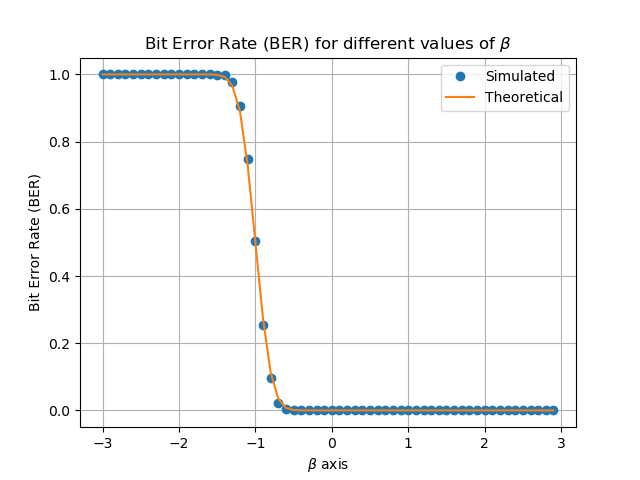
\includegraphics[width=\columnwidth]{Figure_1.png}
%    \caption{Graph of x+y=1}
%    \label{Figure_1}
%\end{figure}
Therefore ,
\begin{align}
    f_{X|Y}\brak{x|y} &= \frac{f_{XY}\brak{x,y}}{f_Y\brak{y}}\\
    & = \frac{ae^{-2y}}{aye^{-2y}}\\
    & = \frac{1}{y}\\
\implies f_{X|Y}\brak{x|y} &=
    \begin{cases}
    \frac{1}{y} & \text{if } 0<x<y<\infty\\
    0 & \text{otherwise}
    \end{cases}
\end{align}
Then, 
\begin{align}
   E\brak{X|Y=y} & =
   \int_{-\infty}^{\infty} (x)f_{X|Y}\brak{x|y}dx\\
    & = \int_{0}^{y}(x)\brak{\frac{1}{y}}dx\\
    & = \frac{1}{y} \int_{0}^{y}(x)dx \\
    & = \frac{1}{y} \left[ \frac{x^2}{2}\right]_{0}^{y}\\
    & = \frac{1}{y}\brak{\frac{y^2}{2}}\\
    & = \frac{y}{2}\\
\implies E\brak{X|Y=y} &= \frac{y}{2}\\
\therefore E\brak{X|Y=2} &= 1
\end{align}
%
\item Let Z be the vertical coordinate, between -1 and 1, of a point chosen uniformly at random on the
\begin{math}
\text{surface of a unit sphere in }R^3.\text{ Then,} \pr{\frac{-1}{2} \leq Z \leq \frac{1}{2}}
\end{math}
is
\\
  \solution
  The equation of the sphere can be written as :
\begin{math}
x^2 + y^2 + z^2 = 1.
\end{math}
Now,
\begin{align}
\pr{\frac{-1}{2} \leq z \leq 0}&=\pr{0 \leq z^2 \leq \frac{1}{4}}
\\\pr{0 \leq z \leq \frac{1}{2}}&=\pr{0 \leq z^2 \leq \frac{1}{4}}
\\\therefore \pr{\frac{-1}{2} \leq z \leq \frac{1}{2}}&=2 \times \pr{0 \leq z^2 \leq \frac{1}{4}}
\end{align}
\begin{align}
\pr{0 \leq z^2 \leq \frac{1}{4}}&=\pr{\frac{3}{4} \leq x^2+y^2 \leq 1}
\\\text{Taking, } x^2+y^2&=r^2.
\end{align}
\begin{align}
     \pr{\frac{3}{4} \leq r^2 \leq 1} &= \frac{1}{4}
\end{align}
     \brak{ \text{Since, }r^2 \text{ is uniform between 0 and 1} }
\begin{align}
     \therefore \pr{\frac{-1}{2} \leq Z \leq \frac{1}{2}} &= 2 \times \frac{1}{4} = \frac{1}{2}
\end{align}

  %
\item Let (X,Y) be a random vector such that, for any $y>0$, the conditional probability density function of X given $Y=y$ is $$f_{X|Y=y}(x)=ye^{-yx} \:,x>0. $$ If the marginal probability density function of Y is $$g(y)=ye^{-y}\:,y>0$$ then $E(Y|x=1)=$
\\
\solution
Given,
the conditional probability density function of X given $Y=y$,
\begin{align}
f_{X|Y=y}(x)=ye^{-yx} \:,x>0 \label{st2020-43:a}
\end{align}
and, the marginal probability density function of Y,
\begin{align}
g(y)=ye^{-y}\:,y>0 \label{st2020-43:b}
\end{align}
let the joint probability density function of (X,Y) be $f_{X,Y}(x,y)$.
We know that,
\begin{align}
f_{X|Y=y}(x)=\frac{f_{X,Y}(x,y)}{g(y)}  \label{st2020-43:c}
\end{align}
using \eqref{st2020-43:a} and \eqref{st2020-43:b} in \eqref{st2020-43:c},
\begin{align}
f_{X,Y}(x,y) =y^{2}e^{-y(x+1)} \:,x,y>0 \label{st2020-43:d}
\end{align}
let the marginal probability density function of X be $f_{X}(x)$,
as we know ,
\begin{align}
f_{X}(x)= \int_{0}^{\infty}{f_{X,Y}(x,y)}\,dy \label{st2020-43:e}
\end{align}
using \eqref{st2020-43:d} in \eqref{st2020-43:e},
\begin{align}
f_{X}(x) &=\int_{0}^{\infty}{y^{2}e^{-y(x+1)}}\,dy\\
&=\frac{2}{(x+1)^{3}} \:,x>0\label{st2020-43:f}
\end{align}
The conditional probability density function of Y given $X=x$ is given by,
\begin{align}
f_{Y|X=x}(y) =\frac{f_{X,Y}(x,y)}{f_{X}(x)} \label{st2020-43:g}
\end{align}
using \eqref{st2020-43:d} and \eqref{st2020-43:f} in \eqref{st2020-43:g},
\begin{align}
 f_{Y|X=x}(y) =\frac{y^{2}e^{-y(x+1)}(x+1)^{3}}{2} \:,x,y>0
\end{align}
The conditional probability density function of Y given $X=1$ is given by,
\begin{align}
 f_{Y|X=1}(y) =4y^{2}e^{-2y}  \:,y>0 \label{st2020-43:h}
\end{align}
We need to find $E(Y|X=1)$ which is given by,
\begin{align}
 E(Y|X=1) &= \int_{0}^{\infty}{yf_{Y|X=1}(y)}\,dy \label{st2020-43:i}
\end{align}
using \eqref{st2020-43:h} in \eqref{st2020-43:i},
\begin{align}
E(Y|X=1) &= \int_{0}^{\infty}{4y^{3}e^{-2y}}\,dy\\
  &= \left[\frac{-e^{-2y}(8y^{3} + 12y^{2} + 12y + 6)}{4}\right]_0^{\infty}\\
        &=\frac{3}{2}
\end{align}

%
%
\item Let $X$ and $Y$ be jointly distributed random
variables having the joint probability
density function
\[
f(x,y) = \begin{cases}
            \frac{1}{\pi}, &\text{if}\quad x^2 + y^2 \leq 1\\
             0, &\text{otherwise}\\
            \end{cases}
\]
Then $\pr{Y > \text{max}(X,-X)}$ is
\\
\solution 

The pdf of $X$ and $Y$ are:
\begin{align}
    f_X(x)&=\int_{-\infty}^{\infty}f(x,y)dy\\
    &=\int_{-\sqrt{1-x^2}}^{\sqrt{1-x^2}}\frac{1}{\pi}dy\\
    &=\frac{2\sqrt{1-x^2}}{\pi}
\end{align}
\begin{align}
    f_Y(y)&=\int_{-\infty}^{\infty}f(x,y)dx\\
    &=\int_{-\sqrt{1-y^2}}^{\sqrt{1-y^2}}\frac{1}{\pi}dx\\
    &=\frac{2\sqrt{1-y^2}}{\pi}
\end{align}
The cdf of $Y$ is:
\begin{align}
    F_Y(y)&=\int_{-\infty}^{y}f_Y(y)dy\\
    &=\int_{-1}^{y}\frac{2\sqrt{1-y^2}}{\pi}dy\\
    &=\frac{2}{\pi}\left(\dfrac{\sin^{-1}{y} + y\sqrt{1-y^2}}{2} + \frac{\pi}{4}\right)
\end{align}
The value of $\pr{-X<Y<X}$ is:
\begin{align}
\pr{-X<Y<X} &=F_Y(X)-F_Y(-X)\\
 &=\frac{2}{\pi}\left(\sin^{-1}{X} + X\sqrt{1-X^2}\right)
\end{align}
Integrating our probability over all of $X$ we get the value of $ E[\pr{-x<Y<x}]$:
\begin{align}
&=\int_{-\infty}^{\infty}f_X(x)\pr{-x<Y<x}dx\\
    &=\left(\frac{2}{\pi}\right)^2\int_0^1\sqrt{1-x^2}\left(\sin^{-1}{x} + x\sqrt{1-x^2}\right)dx
\end{align}
Substituting
\begin{align} 
u &= \sin^{-1}{x} + x\sqrt{1-x^2}\\
\frac{du}{dx} &= 2\sqrt{1-x^2}\\
&=\left(\frac{2}{\pi}\right)^2\int_0^{\frac{\pi}{2}}\frac{u}{2}du\\
&=\left(\frac{2}{\pi}\right)^2\left(\frac{u^2}{4} \bigg |_0^{\frac{\pi}{2}}\right)\\
&=\left(\frac{2}{\pi}\right)^2\left(\frac{\pi^2}{16} - 0\right)\\
    &=\frac{4\cdot{\pi}^2}{{\pi}^2\cdot16}\\
    &=\frac{1}{4}
\end{align}
The probability for:
\begin{align}
    \pr{Y>\text{max}(X,-X)} = \frac{1}{4}
\end{align}
%
\item Let $X$ and $Y$ be two continuous random variables with the joint probability density function
\begin{align}
    f(x,y) =
    \begin{cases}
    2, & 0<x+y<1, x>0, y>0,\\
    0, & elsewhere.
    \end{cases}
\end{align}
$E\brak{X \bigm| Y=\frac{1}{2}}$ is
\begin{enumerate}
    \item $1/4$
    \item $1/2$
    \item $1$
    \item $2$
\end{enumerate}
\solution
%We know that,
\begin{align}
\phi_X(t) &= \int_\mathbb{R} e^{itx}f_X(x) \; dx\\
\phi_X(2\pi) &= \int_\mathbb{R} e^{2\pi ix}f_X(x) \; dx\\
&= \int_\mathbb{R} \cos(2\pi x) f_X(x) \; dx \nonumber \\
&+ i \int_\mathbb{R} \sin(2 \pi x) f_X(x) \; dx \\
\because \phi_X(2\pi) = 1, & \int_\mathbb{R} \sin(2 \pi x) f_X(x) \; dx = 0\\
1 &= \phi_X(2\pi)\\
&= \int_\mathbb{R} \cos(2\pi x) f_X(x) \; dx
\end{align}
Assume that $\cos(2\pi x) \neq 1$. This implies that $\cos(2\pi x) < 1 \; \forall \; x \in \mathbb{R}$.
\begin{align}
\therefore 1 &= \int_\mathbb{R} \cos(2\pi x) f_X(x) \; dx \\
&< \int_\mathbb{R} 1 \cdot f_X(x) \; dx \\
&< \int_\mathbb{R} f_X(x) \; dx \\
&< 1. \tag{Contradiction}
\end{align}
Hence, our assumption that $\cos(2\pi x) \neq 1$ is incorrect.
\begin{align}
&\therefore \cos(2 \pi x) = 1, \; \text{for all  $X=x$}\\
&\Rightarrow X \in \; \mathbb{Z}\\
&\Rightarrow \pr{X \in \mathbb{Z}} = 1
\end{align}

%
\item Let $X ,Y$ be continuous random variables with joint density function
\begin{align*}
    f_{X,Y}(x,y)=\begin{cases}
    e^{-y}(1-e^{-x}) \text{   if } 0< x<y<\infty\\
    e^{-x}(1-e^{-y}) \text{   if } 0< y\leq x<\infty
    \end{cases}
\end{align*}
Then The value of $E[X+Y]$ is 
%
\solution
  Let $g(X,Y)=X+Y$
We know that,
\begin{align*}
    &E[g(X,Y)]=\int_{-\infty}^{+\infty}\int_{-\infty}^{+\infty}g(x,y)f_{X,Y}(x,y)dxdy\\
\end{align*}
Then,
\begin{align*}
    &E[X+Y]=\int_{-\infty}^{+\infty}\int_{-\infty}^{+\infty}(x+y)f_{X,Y}(x,y)\,dxdy\\
    &=\int_{0}^{+\infty}\int_{0}^{+\infty}(x+y)f_{X,Y}(x,y)\,dxdy\\
    &=\int_{0}^{+\infty}\left(\int_{0}^{+\infty}xf_{X,Y}(x,y)\,dx+\int_{0}^{+\infty}yf_{X,Y}(x,y)\,dx\right)\,dy
\end{align*}
First we will calculate the $\int_{0}^{+\infty}yf_{X,Y}(x,y)\,dx$,  $\int_{0}^{+\infty}xf_{X,Y}(x,y)\,dx$ seperately.\\
consider,
\begin{align*}
    &\int_{0}^{+\infty}yf_{X,Y}(x,y)\,dx\\
    &=\int_{0}^{y}ye^{-y}(1-e^{-x})\,dx+\int_{y}^{+\infty}ye^{-x}(1-e^{-y})\,dx\\
    &=(ye^{-y})(y+e^{-y}-1)+y(1-e^{-y})e^{-y}\\
    &=y^2e^{-y}
\end{align*}
So,
\begin{align}
    \tag{37.1}
    \int_{0}^{+\infty}yf_{X,Y}(x,y)\,dx=y^2e^{-y}
\end{align}
Now consider,
\begin{align*}
  &\int_{0}^{+\infty}xf_{X,Y}(x,y)\,dx\\
  &=\int_{0}^{y}xe^{-y}(1-e^{-x})\,dx+\int_{y}^{+\infty}xe^{-x}(1-e^{-y})\\
  &=e^{-y}\left(\frac{y^2}{2}+e^{-y}(y+1)-1\right)+(1-e^{-y})(e^{-y}(y+1))\\
  &=\frac{y^2e^{-y}}{2}+ye^{-y}
\end{align*}
So,
\begin{align}
    \tag{37.2}
    \int_{0}^{+\infty}xf_{X,Y}(x,y)\,dx=\frac{y^2e^{-y}}{2}+ye^{-y}
\end{align}
From Eq 37.1 and 37.2
\begin{align*}
    &E[X+Y]=\int_{0}^{+\infty}\left(\frac{y^2e^{-y}}{2}+ye^{-y}+y^2e^{-y}\right)\,dy\\
    &=\int_{0}^{+\infty}\left(\frac{3}{2}y^2e^{-y}+ye^{-y}\right)\,dy\\
    &=\left(-\frac{3}{2}(y^2+2y+2)e^{-y}+(-e^{-y}(y+1))\right)\Biggr|_{0}^{+\infty}\\
    &=\frac{3}{2}\times2+1\\
    &=4
\end{align*}
So,
\begin{align*}
  &E[X+Y]=4
\end{align*}
%
\item Let $(X,Y)$ be a two-dimensional random variable such that $E(X)=E(Y)=1/2$, $Var(X)=Var(Y)=1$ and $Cov(X,Y)=1/2$.
Then, $P(|X-Y|>6)$ is
\begin{enumerate}

    \item less than 1/6
    \item equal to 1/2
    \item equal to 1/3
    \item greater than 1/2

\end{enumerate}
\solution
  
Given,
\begin{align} \label{ma2001-24:eq-1}
    E(X)=E(Y)=3
\end{align}
\begin{align}
    Var(X)=Var(Y)=1
\end{align}
\begin{align}
    Cov(X,Y)=1/2
\end{align}
Now,
\begin{align}
    Var(X)=E(X^2)-(E(X))^2
\end{align}
Substituting given values, we get,
\begin{align}
    1=E(X^2)-3^2
\end{align}
So,
\begin{align} \label{ma2001-24:eq-2}
    E(X^2)=10
\end{align}
Similarly for $Y$,
\begin{align} \label{ma2001-24:eq-3}
    E(Y^2)=10
\end{align}
Also,
\begin{align}
    Cov(X,Y)=E(XY)-E(X)E(Y)
\end{align}
Substituting given values, we get,
\begin{align}
    1/2=E(XY)-(3)(3)
\end{align}
So,
\begin{align} \label{ma2001-24:eq-4}
    E(XY)=19/2
\end{align}
Let $Z$ be a random variable defined as
\begin{align} \label{ma2001-24:eq-5}
    Z=X-Y
\end{align}
Then using \eqref{ma2001-24:eq-1},
\begin{align} \label{ma2001-24:eq-6}
    E(Z)=E(X-Y)=E(X)-E(Y)=0
\end{align}
Now, using \eqref{ma2001-24:eq-6}
\begin{align}
    Var(Z)=E(Z^2)-(E(Z))^2=E(Z^2)
\end{align}
\begin{align}
    Var(Z)=E((X-Y)^2)
\end{align}
\begin{align}
    Var(Z)=E(X^2)+E(Y^2)-2E(XY)
\end{align}
Using \eqref{ma2001-24:eq-2}, \eqref{ma2001-24:eq-3} and \eqref{ma2001-24:eq-4},
\begin{align}
    Var(Z)=10+10-2 \times 19/2
\end{align}
\begin{align} \label{ma2001-24:eq-7}
    Var(Z)=1
\end{align}
\begin{theorem}
(Chebychev's Inequality)\ Let T be an arbitrary random variable, with finite mean E(T), then for all $a>0$,
\begin{align}
    \pr{|T-E(T)| \geq a} \leq \dfrac{Var(T)}{a^2}
\end{align}
\end{theorem}
\begin{proof}
Let $A$ be a non-negative random variable and $a>0$ be any real number. Define a new random variable $B$ by
\begin{align}
B=  \begin{cases} 
          a & A \geq a \\
          0 & A < a
    \end{cases}
\end{align}
Then clearly $B \leq A$ and by monotonicity,
\begin{align} \label{ma2001-24:eq-8}
    E(B) \leq E(A)
\end{align}
\begin{align}
    E(B)=a\pr{B=a}+0\pr{B=0}
\end{align}
\begin{align} \label{ma2001-24:eq-9}
    E(B)=a\pr{A \geq a}
\end{align}
By \eqref{ma2001-24:eq-8} and \eqref{ma2001-24:eq-9},
\begin{align}
    a\pr{A \geq a} \leq  E(A)
\end{align}
\begin{align} \label{ma2001-24:eq-10}
    \pr{A \geq a} \leq \dfrac{E(A)}{a}
\end{align}
Set $A=(T-E(T))^2$. Then,
\begin{align}
    \pr{|T-E(T)| \geq a}=\pr{A \geq a^2}
\end{align}
Using \eqref{ma2001-24:eq-10},
\begin{align}
    \pr{|T-E(T)| \geq a} \leq \dfrac{E(A)}{a^2}
\end{align}
\begin{align}
    \pr{|T-E(T)| \geq a} \leq \dfrac{E(T-E(T))^2}{a^2}
\end{align}
\begin{align}
    \pr{|T-E(T)| \geq a} \leq \dfrac{Var(T)}{a^2}
\end{align}
\end{proof}
Applying Chebychev's Inequality for $Z$ with $a=6$, we get,
\begin{align}
    \pr{|Z-E(Z)| \geq 6} \leq \dfrac{Var(Z)}{6^2}
\end{align}
Using \eqref{ma2001-24:eq-6} and \eqref{ma2001-24:eq-7},
\begin{align}
    \pr{|Z-0| \geq 6} \leq \dfrac{1}{36}
\end{align}
As $Z=X-Y$,
\begin{align}
    \pr{|X-Y| \geq 6} \leq \dfrac{1}{36}
\end{align}
  \item The variable $x$ takes a value between $0$ and $10$ with uniform probability distribution. The variable $y$ takes a value between $0$ and $20$ with uniform probability distribution.The probability that sum of variables $(x+y)$ being greater than $20$ is
%
\item Let (X,Y) be the coordinates of a point chosen at random inside the disc $x^2 + y^2 \leq r^2$ where $r\geq 0$. The probability that $Y \geq mX$ is
\begin{enumerate}[label = (\alph*)]
\setlength\itemsep{2em}
    \item $\dfrac{1}{2^r}$
    \item $\dfrac{1}{2^m}$
    \item $\dfrac{1}{2}$
    \item $\dfrac{1}{2^{r+m}}$
\end{enumerate}
%
\solution
  
We know that the point $(X,Y)$ satisfies the equation 
\begin{align}
x^2 + y^2 \leq r^2 
\end{align}
Let a random variable $Z\in \{0,1\}$ denote the possible outcomes of the experiment
\begin{table}[h]
\centering
    \begin{tabular}{|c|c|}
        \hline
        Equation satisfied by (X,Y)& Z    \\\hline
        $y-mx<0$ & 0    \\\hline
        $y-mx\geq0$ & 1 \\\hline
    \end{tabular}
\caption{Outcome of the Experiment}
\label{ma2001-2.23:table=1}
\end{table}

The coordinates $(X,Y)$ can be parametrized as follows:
\begin{align}
    X = a\sin\theta\\
    Y = a\cos\theta
\end{align} 
where $a \in [0,r]$ and $\theta \in [0, 2\pi]$. 
\begin{align}
    Y &\geq mX\\
    \implies a\sin\theta &\geq ma\cos\theta
\end{align}

\begin{figure}[h]
    \centering
    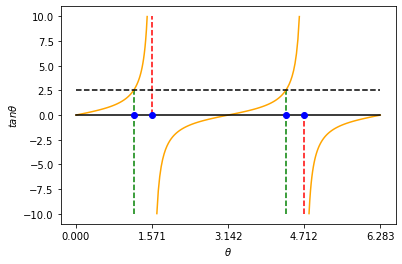
\includegraphics[width=\columnwidth]{solutions/adv/ma/2001/2.23/figures/tanx.png}
    \caption{$tan\theta$ with $m=2.5$}
    \label{ma2001-2.23:tanx}
\end{figure}

This gives two cases for an arbitrary value of $m$ (as seen in fig \ref{ma2001-2.23:tanx}):
\begin{enumerate}
    \item when $\theta\in \left[0,\dfrac{\pi}{2}\right]\cup\left[\dfrac{3\pi}{2},2\pi\right]$, from \ref{ma2001-2.23:tanx},
    \begin{align}
        \tan\theta&\geq m\\
        \implies \theta &\in [\tan^{-1}m, \pi/2]
    \end{align}
    \item similarly, when $\theta \in \left[\dfrac{\pi}{2}, \dfrac{3\pi}{2}\right]$
    \begin{align}
        \tan\theta&\leq m\\
        \implies \theta &\in [\pi/2, \pi+\tan^{-1}m]
    \end{align}
\end{enumerate}
\begin{align}
    \therefore \theta &\in [\tan^{-1} m, \pi+\tan^{-1} m]
\end{align}

$\theta$ will have a uniform probability distribution function: 
\begin{align}
    f(\theta)=\nonumber
    \begin{cases}
    0 &\text{if } \theta<0\\
    \dfrac{1}{2\pi} & \text{if } 0\leq\theta\leq2\pi\\
    0 &\text{if } \theta>2\pi
    \end{cases}
\end{align}
The shaded region of figure \ref{ma2001-2.23:fig:my_label} represents the required probability. 
\begin{align}
    \pr{\arctan m\leq\theta\leq\tan^{-1} m +\pi}\nonumber\\
    =\displaystyle\int\limits_{\tan^{-1} m}^{\pi + \tan^{-1} m} f(\theta) \,d\theta
\end{align}
\begin{align}
    &=\displaystyle\int\limits_{\tan^{-1} m}^{\pi + \tan^{-1} m} \frac{1}{2\pi} \,d\theta\\
    &=\frac{\pi}{2\pi}\\
    &=\frac{1}{2}
\end{align}
\begin{figure}[h!]
    \centering
    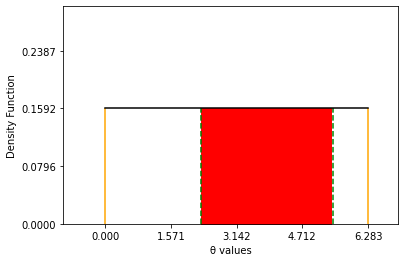
\includegraphics[width=\columnwidth]{solutions/adv/ma/2001/2.23/figures/distribution_2.png}
    \caption{Distribution function of $\theta$}
    \label{ma2001-2.23:fig:my_label}
\end{figure}\\
\\ $\therefore$ option (c) is correct.



%
\item Let $X \sim B(5,\frac{1}{2})$ and $Y \sim U(0,1)$. Then $\frac{P(X + Y \leq 2)}{P(X + Y \geq 5)}$ is equal to 
(where 
$B(n,p)$ : Binomial distribution with n trials and success probability p; $n \in \{1,2, \dots \}$ and  $p \in (0,1)$
U(a,b) : Uniform distribution on the interval $(a,b), -\infty < a < b < \infty$  )
\\
\solution
  Given X is a Binomial Random Variable with 5 trails and success probability $p=0.5$ and Y is a Continuous Random Variable over the interval $(0,1)$.
So, $X \in \{0,1,2,3,4,5\}$ and $Y = U(0,1)$
Since X and Y are Independent Random Variables,
\begin{align}
\pr{X + Y \leq 2} &= \pr{X = a, Y \leq 2-a} \\
&= \sum_{a = 0}^{a = 2} \pr{X = a}\pr{Y \leq 2-a} 
\end{align}
\begin{multline}
\pr{X + Y \leq 2} = \pr{X = 0}\pr{Y \leq 2} \label{ma2015-8:0.0.3} \\ 
+ \pr{X = 1}\pr{Y \leq 1} + \pr{X = 2}\pr{Y \leq 0}    
\end{multline}
Since $X$ is a Binomial Random Variable,
\begin{align}
\pr{X = k} = \begin{cases}
\comb{n}{k}p^{n-k}(1-p)^{k} & 0 \leq k \leq 5 \\
0 & otherwise
\end{cases} \label{ma2015-8:0.0.4}
\end{align}
Substituting the values of n = 5 and p = $\frac{1}{2}$ in \eqref{ma2015-8:0.0.4}, we get
\begin{align*}
\pr{X = k} = \comb{5}{k} \left(\frac{1}{2} \right)^{5-k} \left(\frac{1}{2} \right)^{k} = \comb{5}{k} \left(\frac{1}{2} \right)^{5}    
\end{align*}
Also, the Cumulative Distribution Function of $Y$ is
defined as
\begin{align}
CDF(Y) = F_Y(a) = \pr{Y \leq a} = \begin{cases}
0 & a \leq 0 \\
a & 0 < a < 1 \\ 
1 & a \geq 1
\end{cases} \label{ma2015-8:0.0.5}   
\end{align}
By substituting the probability values from \eqref{ma2015-8:0.0.4} and \eqref{ma2015-8:0.0.5} in \eqref{ma2015-8:0.0.3}, we get
\begin{multline}
\pr{X + Y \leq 2} = \comb{5}{0} \left(\frac{1}{2} \right)^{5}(1) + \comb{5}{1} \left(\frac{1}{2} \right)^{5}(1) \\ + \comb{5}{2} \left(\frac{1}{2} \right)^{5}(0)    
\end{multline}
\begin{align}
&= (1)\left(\frac{1}{32} \right) + (5)\left(\frac{1}{32} \right) + 0 \\
&= \left(\frac{1}{32} \right) + \left(\frac{5}{32} \right) \\
&= \frac{6}{32} \\
\pr{X + Y \leq 2} &= \frac{3}{16}    
\end{align}
Now,
\begin{align}
\pr{X + Y \geq 5} &= 1 - \pr{X + Y <  5}
\end{align}
\begin{multline}
= 1 - [\pr{X + Y \leq 5} - \\ \pr{X + Y = 5}] \label{ma2015-8:0.0.12}    
\end{multline}
But, as Y is a Continuous Random Variable over $(0,1)$, so $\pr{Y = k } = 0$  $\forall$ k $\in [0,1]$ . Therefore considering all possible cases,
\begin{multline}
\pr{X + Y = 5} = \pr{X = 4}\pr{Y = 1} \\ + \pr{X = 5}\pr{Y = 0}    
\end{multline}
\begin{align}
&= \pr{X = 4}(0) + \pr{X = 5}(0) \\
&= 0 + 0 
\end{align}
\begin{align}
\pr{X + Y = 5} &= 0 \label{ma2015-8:0.0.16}    
\end{align}
Hence, by substituting \eqref{ma2015-8:0.0.16} in \eqref{ma2015-8:0.0.12}, we get
\begin{align}
\pr{X + Y \geq 5} &= 1 - [\pr{X + Y \leq 5} -  0] \\
\pr{X + Y \geq 5} &= 1 - \pr{X + Y \leq 5} \\
\pr{X + Y \geq 5} &= 1 - \pr{X = a, Y \leq 5 - a}
\end{align}
\begin{align}
&= 1 - \left[\sum_{a = 0}^{a = 5} \pr{X = a}\pr{Y \leq 5-a} \right]     
\end{align}
\begin{multline}
= 1 - [ \pr{X = 0}\pr{Y \leq 5} + \pr{X = 1}\pr{Y \leq 4} \\
+ \pr{X = 2}\pr{Y \leq 3} + \pr{X = 3}\pr{Y \leq 2} \\
+ \pr{X = 4}\pr{Y \leq 1} + \pr{X = 5}\pr{Y \leq 0} ] \label{ma2015-8:0.0.21}    
\end{multline}
By substituting the probability values from \eqref{ma2015-8:0.0.4} and \eqref{ma2015-8:0.0.5} in \eqref{ma2015-8:0.0.21}, we get
\begin{multline}
\pr{X + Y \geq 5} = 1 - [\comb{5}{0}\left(\frac{1}{2}\right)^{5}(1) + \comb{5}{1}\left(\frac{1}{2}\right)^{5}(1) + \\ \comb{5}{2}\left(\frac{1}{2}\right)^{5}(1) + 
\comb{5}{3}\left(\frac{1}{2}\right)^{5}(1) + \\
\comb{5}{4}\left(\frac{1}{2}\right)^{5}(1) + 
\comb{5}{5}\left(\frac{1}{2}\right)^{5}(0)]  
\end{multline}
\begin{multline}
\pr{X + Y \geq 5} = 1 - \left(\frac{1}{2}\right)^{5} [\comb{5}{0} + \comb{5}{1} \\ + \comb{5}{2} + \comb{5}{3} + \comb{5}{4}]    
\end{multline}
\begin{align}
&= 1 - \left(\frac{1}{32}\right)\left[1 + 5 + 10 + 10 + 5 \right] \\
&= 1- \left(\frac{1}{32}\right)\left[31 \right] = \frac{1}{32}
\end{align}
Hence,
$\pr{X + Y \leq 2} = \frac{3}{16}$ and $\pr{X + Y \geq 5} = \frac{1}{32}$.
\begin{align*}
\therefore \frac{\pr{X + Y \leq 2}}{\pr{X + Y \geq 5}} = \frac{\frac{3}{16}}{\frac{1}{32}} = 6. \\
\therefore \frac{\pr{X + Y \leq 2}}{\pr{X + Y \geq 5}} = 6    
\end{align*}
Hence, the required ratio is 6 .



\end{enumerate}